\documentclass{article}
\usepackage[utf8]{inputenc}
\usepackage{amsmath}
\usepackage{amssymb}
\usepackage{graphicx}
\usepackage{listings}



\begin{document}

\section*{Householder reflections}
\subsection*{1-5.a}
We are given the following algorithm to construct a Householder reflection.
\begin{figure}[!hbt]
    \centering
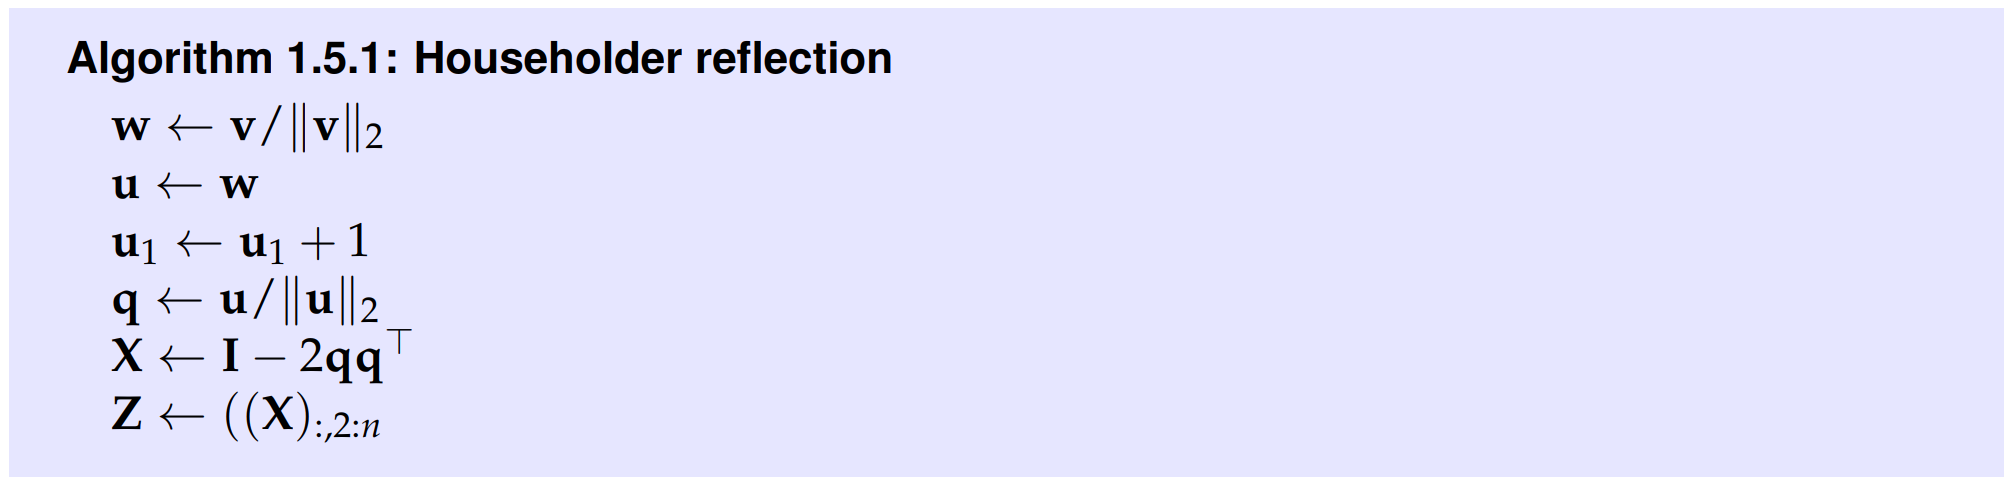
\includegraphics[width=1.0\linewidth]{HouseholderReflections.png}
\end{figure}

\noindent This leads to the following code.

\begin{figure}[!hbt]
    \centering
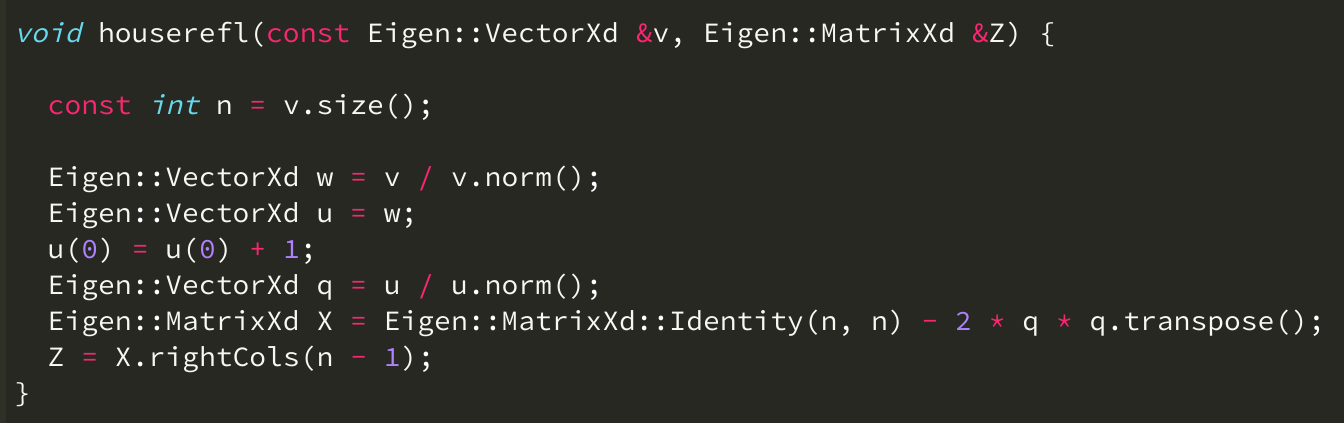
\includegraphics[width=1.0\linewidth]{1-5.a.png}
\end{figure}

\noindent Instead of using \verb|v / v.norm()| one could also use \verb|v.normalized()| but the effect is the same.

\subsection*{1-5.b}
We are now tasked with proving that the matrix $\mathbf{M}$ as defined above satisfies
\begin{equation*}
\mathbf{X}^{\mathsf{T}}\mathbf{X} = \mathbf{I}_{n}
\end{equation*}
We will go through this step by step. First we take the input vector \verb|v| and compute
\begin{equation*}
    \mathbf{w} = \frac{\mathbf{v}}{\left\lVert \mathbf{v} \right\rVert_{2}}
\end{equation*}

In a next step we do \verb|u = w| and then add $1$ the first entry of \verb|u|.
\begin{equation*}
    \mathbf{u} = 
    \begin{bmatrix}
    w_{0} + 1 \\
    w_{1} \\
    \vdots \\
    w_{n - 1}
    \end{bmatrix} = 
    \begin{bmatrix}
      w_{0} \\
    w_{1} \\
    \vdots \\
    w_{n - 1}  
    \end{bmatrix} + 
    \begin{bmatrix}
        1 \\
        0 \\
        \vdots \\
        0
    \end{bmatrix}
    = \mathbf{w} + \mathbf{e}_{1} = \mathbf{w} + \left\lVert \mathbf{w} \right\rVert_{2}\mathbf{e}_{1}
\end{equation*}
This is the case because we just normalized \verb|v| to get \verb|w| and hence $\left\lVert w \right\rVert_{2} = 1$. We now first need to understand some things about the norm. We have
\begin{equation*}
    \left\lVert \mathbf{u} \right\rVert_{2} = \sqrt{u_{1}^{2} + \dots + u_{n}^{2}} = \sqrt{\mathbf{u}^{\mathsf{T}}\mathbf{u}}
\end{equation*} 
What we hence get when doing \verb|q = u / u.norm()| is
\begin{equation*}
   \mathbf{q} = \frac{\mathbf{u}}{\sqrt{\mathbf{u}^{\mathsf{T}}\mathbf{u}}}
\end{equation*}
The next line does \verb|X = I -2qq.transpose()| which is
\begin{align*}
    \mathbf{X} = \mathbf{I} - 2 * \mathbf{q} * \mathbf{q}^{\mathsf{T}} &= \mathbf{I} - 2 * \frac{\mathbf{u}}{\sqrt{\mathbf{u}^{\mathsf{T}}\mathbf{u}}} * \left(\frac{\mathbf{u}}{\sqrt{\mathbf{u}^{\mathsf{T}}\mathbf{u}}}\right)^{\mathsf{T}} \: \text{($\sqrt{\mathbf{u}^{\mathsf{T}}\mathbf{u}}$ is a factor)}\\
   &= \mathbf{I} - 2 * \frac{\mathbf{u}}{\sqrt{\mathbf{u}^{\mathsf{T}}\mathbf{u}}} * \frac{\mathbf{u}^{\mathsf{T}}}{\sqrt{\mathbf{u}^{\mathsf{T}}\mathbf{u}}} \\
    &= \mathbf{I} - 2 * \frac{\mathbf{u}\mathbf{u}^{\mathsf{T}}}{\sqrt{\mathbf{u}^{\mathsf{T}}\mathbf{u}}\sqrt{\mathbf{u}^{\mathsf{T}}\mathbf{u}}} \\
    &= \mathbf{I} - 2 * \frac{\mathbf{u}\mathbf{u}^{\mathsf{T}}}{\mathbf{u}^{\mathsf{T}}\mathbf{u}}
\end{align*}
This now looks very much like the \textbf{Householder reflection} in the same script. We now have
\begin{equation*}
    \mathbf{X} = \mathbf{I} - 2 * \frac{\mathbf{u}\mathbf{u}^{\mathsf{T}}}{\mathbf{u}^{\mathsf{T}}\mathbf{u}}
\end{equation*}
We hence have
\begin{align*}
\mathbf{X}^{\mathsf{T}}\mathbf{X} &= \left(\mathbf{I} - 2 * \frac{\mathbf{u}\mathbf{u}^{\mathsf{T}}}{\mathbf{u}^{\mathsf{T}}\mathbf{u}}\right)^{\mathsf{T}}\left(\mathbf{I} - 2 * \frac{\mathbf{u}\mathbf{u}^{\mathsf{T}}}{\mathbf{u}^{\mathsf{T}}\mathbf{u}}\right) = \left(\mathbf{I}^{\mathsf{T}} - 2 *  \left(\frac{\mathbf{u}\mathbf{u}^{\mathsf{T}}}{\mathbf{u}^{\mathsf{T}}\mathbf{u}}\right)^{\mathsf{T}}\right)\left(\mathbf{I} - 2 * \frac{\mathbf{u}\mathbf{u}^{\mathsf{T}}}{\mathbf{u}^{\mathsf{T}}\mathbf{u}}\right) \\
&= \left(\mathbf{I} - 2 *  \frac{\left(\mathbf{u}\mathbf{u}^{\mathsf{T}}\right)^{\mathsf{T}}}{\mathbf{u}^{\mathsf{T}}\mathbf{u}}\right)\left(\mathbf{I} - 2 * \frac{\mathbf{u}\mathbf{u}^{\mathsf{T}}}{\mathbf{u}^{\mathsf{T}}\mathbf{u}}\right) 
 = \mathbf{I}^{2} - 4\frac{\mathbf{u}\mathbf{u}^{\mathsf{T}}}{\mathbf{u}^{\mathsf{T}}\mathbf{u}} + 4\left(\frac{\mathbf{u}\mathbf{u}^{\mathsf{T}}}{\mathbf{u}^{\mathsf{T}}\mathbf{u}}\right)^{2} \quad \text{($\mathbf{u}^{\mathsf{T}}\in \mathbb{R}$, $\mathbf{u}\mathbf{u}^{\mathsf{T}}$ and $\mathbf{I}$ are symmetric)} \\
&= \mathbf{I}^{2} - 4\frac{\mathbf{u}\mathbf{u}^{\mathsf{T}}}{\mathbf{u}^{\mathsf{T}}\mathbf{u}} + 4\left(\mathbf{q}\mathbf{q}^{\mathsf{T}}\right)^{2} \\
&= \mathbf{I}^{2} - 4\frac{\mathbf{u}\mathbf{u}^{\mathsf{T}}}{\mathbf{u}^{\mathsf{T}}\mathbf{u}} + 4\left(\mathbf{q}\underbrace{\mathbf{q}^{\mathsf{T}}\mathbf{q}}_{= \left\lVert\mathbf{q}\right\rVert = 1}\mathbf{q}^{\mathsf{T}}\right)
\\
&= \mathbf{I}^{2} - 4\frac{\mathbf{u}\mathbf{u}^{\mathsf{T}}}{\mathbf{u}^{\mathsf{T}}\mathbf{u}} + 4\left(\mathbf{q}\mathbf{q}^{\mathsf{T}}\right) \\
&=
\mathbf{I}^{2} - 4\frac{\mathbf{u}\mathbf{u}^{\mathsf{T}}}{\mathbf{u}^{\mathsf{T}}\mathbf{u}} + 4\frac{\mathbf{u}\mathbf{u}^{\mathsf{T}}}{\mathbf{u}^{\mathsf{T}}\mathbf{u}}\\
&= \mathbf{I}^{2} = \mathbf{I} = \mathbf{I}_{n}
\end{align*}

\pagebreak

\subsection*{1-5.c}
We are tasked with showing that the first column of $\mathbf{X}$ is a multiple of the vector $v$. For this purpose we again write
\begin{equation*}
    \mathbf{X} = \mathbf{I} - 2 * \frac{\mathbf{u}\mathbf{u}^{\mathsf{T}}}{\mathbf{u}^{\mathsf{T}}\mathbf{u}}
\end{equation*}
We also remember that 
\begin{equation}
    \mathbf{u} = \mathbf{w} + \left\lVert \mathbf{w}\right\rVert_{2}\mathbf{e}_{1} = \mathbf{w} + \left\lVert \mathbf{w}\right\rVert_{2}\begin{bmatrix}
        1 \\
        0 \\
        \vdots  \\
        0
    \end{bmatrix} \quad \text{and }\left\lVert \mathbf{w}\right\rVert_{2} = 1 
\end{equation}
Let us consider the columns of $\mathbf{X}$
\begin{equation*}
    \mathbf{X}_{1} = 
        \mathbf{e}_{1} - 2 \frac{1}{\mathbf{u}^{\mathsf{T}}\mathbf{u}} \left(\mathbf{u}\mathbf{u}^{\mathsf{T}}\right)_{1}
   = 
   \begin{bmatrix}
     1 - 2 \frac{u_{1}u_{1}}{\sum_{i=1}^{n}u_{i}^{2}} \\
     0 - 2 \frac{u_{1}u_{2}}{\sum_{i=1}^{n}u_{i}^{2}} \\
     \vdots \\
     0 - 2 \frac{u_{1}u_{n}}{\sum_{i=1}^{n}u_{i}^{2}}
   \end{bmatrix}
\end{equation*}
We now need to use the fact that (1) holds to get
\begin{equation*}
    \mathbf{X}_{1} =\begin{bmatrix}
     1 - 2 \frac{u_{1}u_{1}}{\sum_{i=1}^{n}u_{i}^{2}} \\
     0 - 2 \frac{u_{1}u_{2}}{\sum_{i=1}^{n}u_{i}^{2}} \\
     \vdots \\
     0 - 2 \frac{u_{1}u_{n}}{\sum_{i=1}^{n}u_{i}^{2}}
   \end{bmatrix}
   = 
   \begin{bmatrix}
      1- 2\frac{\left(w_{1} + 1\right)\left(w_{1} + 1\right)}{\sum_{i=1}^{n}u_{i}^{2}} \\[1mm]
      - 2\frac{\left(w_{1} + 1\right)w_{2}}{\sum_{i=1}^{n}u_{i}^{2}} \\[1mm]
      \vdots \\
      - 2\frac{\left(w_{1} + 1\right)w_{n}}{\sum_{i=1}^{n}u_{i}^{2}}
   \end{bmatrix} =
   \begin{bmatrix}
      \frac{\sum_{i=1}^{n}u_{i}^{2}}{\sum_{i=1}^{n}u_{i}^{2}}- 2\frac{\left(w_{1} + 1\right)\left(w_{1} + 1\right)}{\sum_{i=1}^{n}u_{i}^{2}} \\[1mm]
      - 2\frac{\left(w_{1} + 1\right)w_{2}}{\sum_{i=1}^{n}u_{i}^{2}} \\[1mm]
      \vdots \\
      - 2\frac{\left(w_{1} + 1\right)w_{n}}{\sum_{i=1}^{n}u_{i}^{2}}
   \end{bmatrix}
\end{equation*}
We know need to use that
\begin{align*}
    \sum_{i=1}^{n}u_{i}^{2} &= \left(w_{1} + 1\right)^{2} + w_{2}^{2} + \dots + w_{n}^{2} 
 \\
 &= 2w_{1} + 1 + \left(w_{1}^{2}+ w_{2}^{2} + \dots + w_{n}^{2}\right) \\
 &= 2w_{1} + 1 + \left\lVert \mathbf{w}\right\rVert^{2} \\
 &= 2w_{1} + 1 + \left\lVert \mathbf{w}\right\rVert \quad \text{($ \left\lVert \mathbf{w}\right\rVert = 1$)}  \\
 &= 2\left(w_{1} + 1\right)
\end{align*}
Putting this into the above matrix gives us
\begin{equation*}
    \mathbf{X}_{1} = \begin{bmatrix}
      \frac{\sum_{i=1}^{n}u_{i}^{2}}{\sum_{i=1}^{n}u_{i}^{2}}- 2\frac{\left(w_{1} + 1\right)\left(w_{1} + 1\right)}{\sum_{i=1}^{n}u_{i}^{2}} \\[1mm]
      - 2\frac{\left(w_{1} + 1\right)w_{2}}{\sum_{i=1}^{n}u_{i}^{2}} \\[1mm]
      \vdots \\
      - 2\frac{\left(w_{1} + 1\right)w_{n}}{\sum_{i=1}^{n}u_{i}^{2}}
   \end{bmatrix} = 
  \begin{bmatrix}
    \frac{2\left(w_{1} + 1\right)}{2\left(w_{1} + 1\right)}- 2\frac{\left(w_{1} + 1\right)\left(w_{1} + 1\right)}{2\left(w_{1} + 1\right)} \\[1mm]
      - 2\frac{\left(w_{1} + 1\right)w_{2}}{2\left(w_{1} + 1\right)} \\[1mm]
      \vdots \\
      - 2\frac{\left(w_{1} + 1\right)w_{n}}{2\left(w_{1} + 1\right)}
   \end{bmatrix}
   = 
   \begin{bmatrix}
    \frac{2w_{1} + 2}{2\left(w_{1} + 1\right)}- \frac{2w_{1}^{2} + 4w_{1} + 2}{2\left(w_{1} + 1\right)} \\[1mm]
      - 2\frac{\left(w_{1} + 1\right)w_{2}}{2\left(w_{1} + 1\right)} \\[1mm]
      \vdots \\
      - 2\frac{\left(w_{1} + 1\right)w_{n}}{2\left(w_{1} + 1\right)}
   \end{bmatrix}
   = \begin{bmatrix}
   - \frac{2w_{1}^{2} + 2w_{1}}{2\left(w_{1} + 1\right)} \\[1mm]
      - 2\frac{\left(w_{1} + 1\right)w_{2}}{2\left(w_{1} + 1\right)} \\[1mm]
      \vdots \\
      - 2\frac{\left(w_{1} + 1\right)w_{n}}{2\left(w_{1} + 1\right)}
   \end{bmatrix}
\end{equation*}

This will now give us
\begin{equation*}
    \mathbf{X}_{1} = \begin{bmatrix}
   - 2\frac{w_{1}^{2} + w_{1}}{2\left(w_{1} + 1\right)} \\[1mm]
      - 2\frac{\left(w_{1} + 1\right)w_{2}}{2\left(w_{1} + 1\right)} \\[1mm]
      \vdots \\
      - 2\frac{\left(w_{1} + 1\right)w_{n}}{2\left(w_{1} + 1\right)}
   \end{bmatrix} = 
   \begin{bmatrix}
   - 2\frac{w_{1}\left(w_{1} +1\right)}{2\left(w_{1} + 1\right)} \\[1mm]
      - 2\frac{\left(w_{1} + 1\right)w_{2}}{2\left(w_{1} + 1\right)} \\[1mm]
      \vdots \\
      - 2\frac{\left(w_{1} + 1\right)w_{n}}{2\left(w_{1} + 1\right)}
   \end{bmatrix} = 
   \begin{bmatrix}
   - 2\frac{w_{1}}{2} \\[1mm]
      - 2\frac{w_{2}}{2} \\[1mm]
      \vdots \\
      - 2\frac{w_{n}}{2}
   \end{bmatrix}
   = - \begin{bmatrix}
       w_{1} \\ w_{2} \\ \vdots \\ w_{n}
   \end{bmatrix} = -\mathbf{w}
\end{equation*}
Now we can finally use that
\begin{equation*}
    \mathbf{w} = \frac{\mathbf{v}}{\left\lVert \mathbf{v}\right\rVert}
\end{equation*}
And thus we get
\begin{equation*}
    \mathbf{X}_{1} = -\frac{\mathbf{v}}{\left\lVert \mathbf{v}\right\rVert} = -\frac{1}{\left\lVert \mathbf{v}\right\rVert}\mathbf{v}
\end{equation*}
hence the first column is a multiple of $\mathbf{v}$.
\subsection*{1-5.d}
The set of columns of the matrix $\mathbf{Z}$ are pairwise orthogonal and also normalized, hence they form an orthonormal basis of $\mathbb{R}^{n}$. The function \verb|houserefl| does now construct this matrix, however we did see that $X_{1}$ is a mutliple of $\mathbf{v}$ and thus
\begin{equation*}
    \text{Span}\left(\mathbf{X}_{1}\right) = \text{Span}\left(\mathbf{v}\right)
\end{equation*}
this means that the columns $X_{2}, \dots, X_{n}$ are a orthonormal basis  of the complement of $\text{Span}\left(\mathbf{X}_{1}\right) = \text{Span}\left(\mathbf{v}\right)$
and thus the function \verb|houserefl| computes an orthonormal basis of the complement of the input vector $\mathbf{v}$.
\subsection*{1-5.e}
We are now tasked with computing the asymptotic complexity of the function \verb|houserefl| depending on the length $n$ of the vector $\mathbf{v}$. We will go through the code line per line

\begin{lstlisting}[language=C++,
                   directivestyle={\color{black}}
                   emph={int,char,double,float,unsigned},
                   emphstyle={\color{blue}}
                  ]
void houserefl(const Eigen::VectorXd &v, Eigen::MatrixXd &Z) {
  
   const int n = v.size();
  
 1  Eigen::VectorXd w = v / v.norm();                    O(n)
 2  Eigen::VectorXd u = w;                               O(n)
 3  u(0) = u(0) + 1;                                     O(1)
 4  Eigen::VectorXd q = u / u.norm();                    O(n)
 5  Eigen::MatrixXd X = Eigen::MatrixXd::Identity(n, n)  O(n^2)
                      - 2 * q * q.transpose();           
 6  Z = X.rightCols(n - 1);                              O(n^2)

}
\end{lstlisting}

\pagebreak

\paragraph{Reasoning:} Normalizing a vector can be done in $\mathcal{O}\left(n\right)$ operations as the norm is computed using
\begin{equation*}
    \left\lVert x\right\rVert = \sqrt{\mathbf{x}^{\mathsf{T}}\mathbf{x}}
\end{equation*}
this takes $n$ multiplications and $n-1$ additions and hence in $\mathcal{O}\left(n\right)$. 
The construction of $\mathbf{X}$ is done by construction an identity matrix (either $\mathcal{O}\left(n\right)$  or $\mathcal{O}\left(n^{2}\right)$ depending on how that is done), the product 
\begin{equation*}
    2 * \mathbf{q} * \mathbf{q^{\mathsf{T}}}
\end{equation*}
takes $\mathcal{O}\left(n^{2}\right)$ operations and the subtraction also takes $\mathcal{O}\left(n^{2}\right)$ operations, hence we get $\mathcal{O}\left(n^{2}\right)$ for this step. Combined we get $\mathcal{O}\left(n^{2}\right)$ for the entire method.
\end{document}
